\chapter{Analyse de données}

Les données à dispositions dans la base de donnée qui a été importée à partir du fichier \textit{aventure2014.sql.gz} n'ont pas été utilisées complétement pour ce laboratoire. Uniquement les attributs suivants ont été utilisés :

\begin{itemize}
	\item MaritalStatus
	\item Gender
	\item YearlyIncome
	\item TotalChildren;
	\item EnglishEducation
	\item EnglishOccupation
	\item HouseOwnerFlag
	\item NumberCarsOwned
\end{itemize}


\section{Arbre de décisions}

L'algorithme choisi pour cette méthode de classification a été REPTree. Après avoir effectué plusieurs runs aux paramètres différents, nous avons choisi un des meilleurs de nos tests.

Sur le listing \autoref{lst:reptree_run}, on observe les informations du run choisis ainsi que les attributs sur la base desquels on veut trouver les classes de l'attributs \texttt{EnglishOccupation} qui sont :

\begin{itemize}
	\item Professional
	\item Management
	\item Skilled Manual
	\item Clerical
	\item Manual
\end{itemize}

\begin{figure}[H]
\centering
\begin{lstlisting}
Scheme:       weka.classifiers.trees.REPTree -M 2 -V 0.001 -N 10 -S 42 -L -1 -P -I 0.0 -batch-size 200
Relation:     QueryResult-weka.filters.unsupervised.attribute.Remove-R1-7,9,11,14,16,18,21-25
Instances:    18484
Attributes:   8
              MaritalStatus
              Gender
              YearlyIncome
              TotalChildren
              EnglishEducation
              EnglishOccupation
              HouseOwnerFlag
              NumberCarsOwned
Test mode:    split 80.0% train, remainder test
\end{lstlisting}
\caption{Information du run REPTree}
\label{lst:reptree_run}
\end{figure}

Le résultat de ce run à montré que la moyenne pondérée des instances correctement classifiées est 91.29\%. La valeur de ce résultat est bonne et indique que notre modèle est bon. Cependant, seul ce résultat ne permet pas d'affirmer que le modèle est bon. Il est nécessaire d'observer les différentes métriques dans la partie \texttt{Detailed Accuracy By Class} du listing \autoref{lst:reptree_res} pour en savoir d'avantage. Sur ce dernier, on constate que \texttt{0.913} est la moyenne des métriques TP Rate, Precision, Recall et F-Measure pour les différentes classes. Notre analyse est donc confortée par la stabilité du résultat moyen de ces différentes métriques.

Maintenant, il est intéressant de savoir quelles sont les forces et faiblesses de notre modèle. Pour cela, nous baserons nos constats sur la F-Measure. Cette dernière étant robuste car elle prend en compte precision et recall. On y voit que la classe au meilleur score est \texttt{Manual} avec 0.970 et la moins bonne est \texttt{Skilled Manual} avec 0.882.

Afin d'améliorer notre modèle, on se concentrera donc sur la classes \texttt{Skilled Manual}. La matrice de confusion nous donne le détail de classification des instances de \texttt{Skilled Manual}. On y voit que \texttt{Skilled Manual} est souvent pris pour \texttt{Professional} et vis et versa. Ceci peut nous donner une piste pour de plus amples analyse ou on se questionnera sur les similarités et différences entre 2 instances de chacune des classes pour comprendre quel sont les facteurs qui rentrent en jeux.

\begin{figure}[H]
\centering
\begin{lstlisting}
=== Summary ===

Correctly Classified Instances        3375               91.2902 %
Incorrectly Classified Instances       322                8.7098 %
Kappa statistic                          0.8883
Mean absolute error                      0.0434
Root mean squared error                  0.1549
Relative absolute error                 13.8991 %
Root relative squared error             39.2271 %
Total Number of Instances             3697

=== Detailed Accuracy By Class ===

TP Rate  FP Rate  Precision  Recall   F-Measure  MCC      ROC Area  PRC Area  Class
0.904    0.043    0.899      0.904    0.902      0.860    0.982     0.963     Professional
0.912    0.019    0.909      0.912    0.910      0.892    0.992     0.970     Management
0.873    0.035    0.892      0.873    0.882      0.844    0.981     0.945     Skilled Manual
0.946    0.013    0.930      0.946    0.938      0.927    0.991     0.971     Clerical
0.972    0.005    0.968      0.972    0.970      0.966    0.997     0.981     Manual

Weighted Avg.

0.913    0.027    0.913      0.913    0.913      0.885    0.987     0.963

=== Confusion Matrix ===

    a    b    c    d    e   <-- classified as
 1002   25   69   12    0 |    a = Professional
   46  568    9    0    0 |    b = Management
   62   32  802   20    3 |    c = Skilled Manual
    4    0   15  545   12 |    d = Clerical
    0    0    4    9  458 |    e = Manual
\end{lstlisting}
\caption{Résultat du run REPTree}
\label{lst:reptree_res}
\end{figure}

Concernant l'arbre de décision, son début est visible dans le listing \autoref{lst:reptree_sample}. Sur cet exemple, on voit que la division commence par l'apport financier, puis l'éducation, les enfants, l'état civil et la possession d'une maison.

Il est intéressant de noter que juste après la division homme-femme, l'état civil et la possession d'une maison ont été interverti dans la branche M et F. Ceci met en évidence que la meilleure manière de diviser les classes est prise en compte en fonction de chacune des instances.

\begin{figure}[H]
\centering
\begin{lstlisting}
YearlyIncome < 45000
|   YearlyIncome < 25000
|   |   EnglishEducation = Bachelors
|   |   |   YearlyIncome < 15000
|   |   |   |   TotalChildren < 1.5
|   |   |   |   |   Gender = M
|   |   |   |   |   |   MaritalStatus = M
|   |   |   |   |   |   |   HouseOwnerFlag = 1 : Manual (27/1) [0/0]
|   |   |   |   |   |   |   HouseOwnerFlag = 0 : Manual (3/0) [0/0]
|   |   |   |   |   |   MaritalStatus = S : Manual (11/0) [0/0]
|   |   |   |   |   Gender = F
|   |   |   |   |   |   HouseOwnerFlag = 1
|   |   |   |   |   |   |   MaritalStatus = M : Manual (21/1) [0/0]
|   |   |   |   |   |   |   MaritalStatus = S : Manual (7/0) [0/0]
|   |   |   |   |   |   HouseOwnerFlag = 0 : Manual (8/1) [0/0]
\end{lstlisting}
\caption{Début du REPTree}
\label{lst:reptree_sample}
\end{figure}


\section{Clustering}

%TODO

\section{Règles d'associations}

Pour cette section, le filtre \textit{NumericToNominal} a été appliqué aux attributs \textit{NumberCarsOwned}, \textit{YearlyIncome} et \textit{TotalChildren}.

Seul les algorithmes \textit{Apriori} et \textit{FilteredAssociator} ont été testé. Seul ceux-ci étaient disponible (voir \ref{associate}).

\begin{figure}[H]
    \centering
    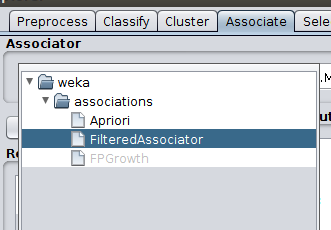
\includegraphics[width=0.5\linewidth, fbox]{img/associate.png}
    \caption{Règles d'associations : Algos disponible}
    \label{associate}
\end{figure}

\subsection{Apriori}

Le seuil minimum de confiance a été modifié pour obtenir plus de règles.

Voici les paramètres :

\begin{lstlisting}
Apriori -N 10 -T 0 -C 0.8 -D 0.05 -U 1.0 -M 0.1 -S -1.0 -c 1
\end{lstlisting}

Et le résultat (figure \ref{apriori}).

\begin{figure}[H]
    \centering
	\makebox[\textwidth][c]{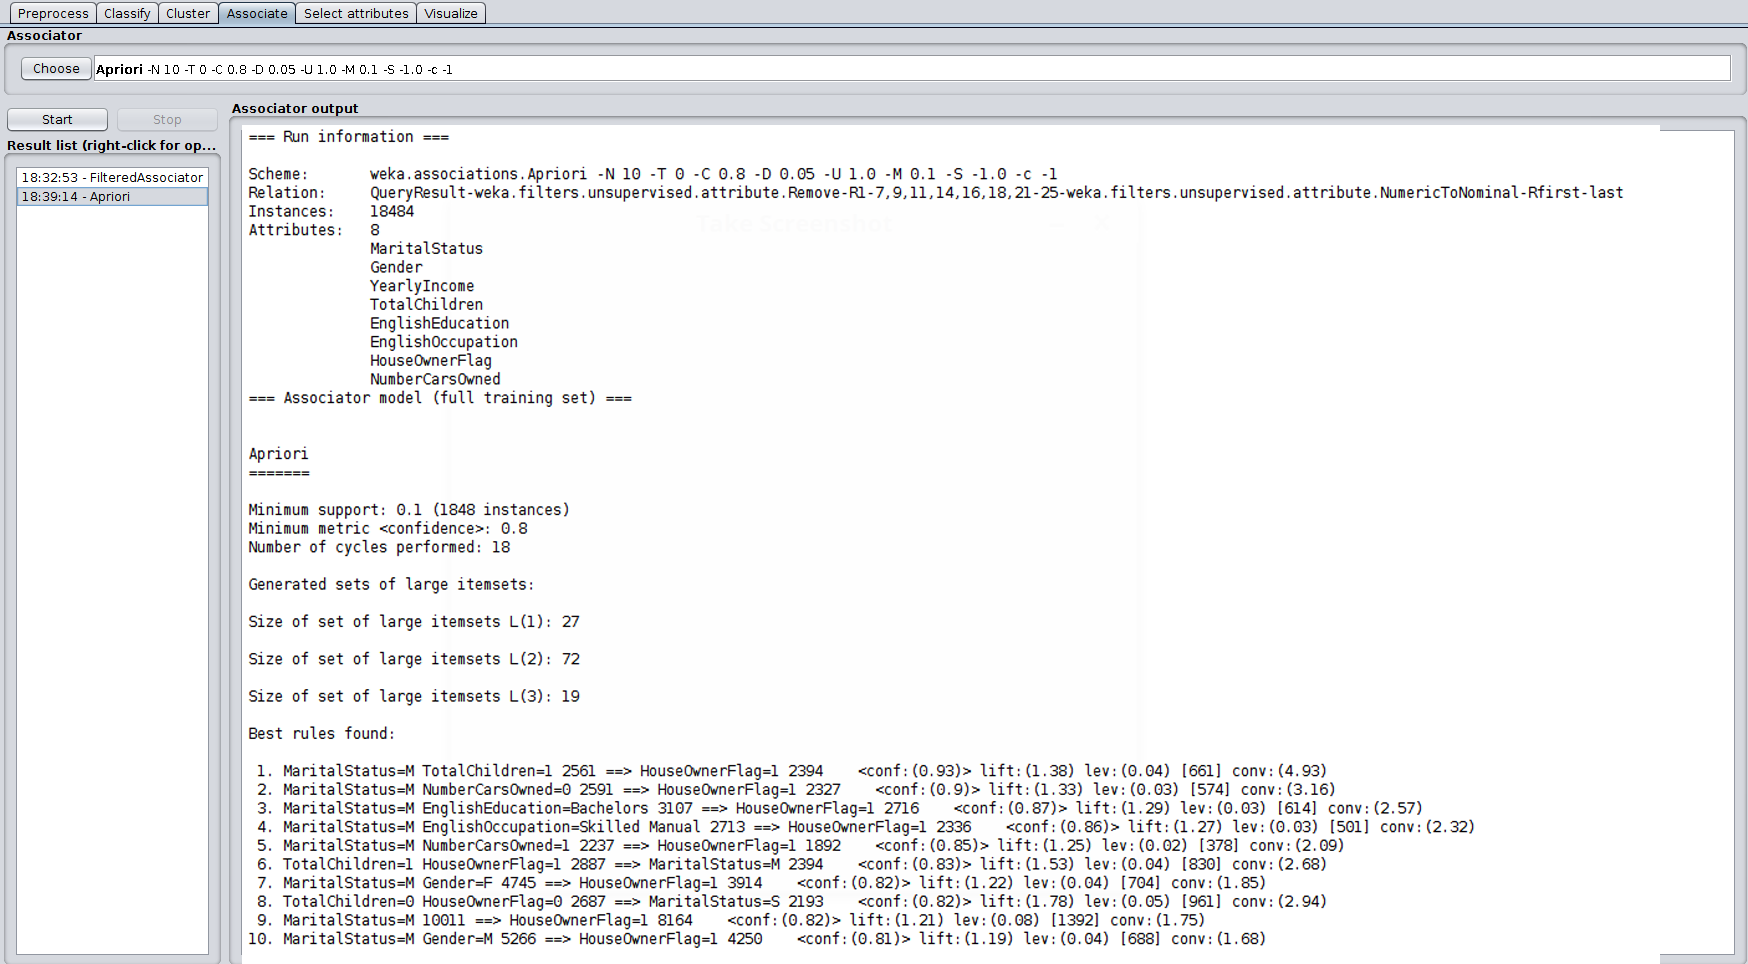
\includegraphics[width=1.3\linewidth, fbox]{img/apriori.png}}%
    \caption{Règles d'associations : Apriori résultat}
    \label{apriori}
\end{figure}

\subsection{FilteredAssociator}

Cet algorithme permet de créer des règles d'association filtrées.

Les 10 règles obtenues (figure \ref{filtered}) sont identiques au résultat de l'\textit{Apriori}.

\begin{figure}[H]
    \centering
	\makebox[\textwidth][c]{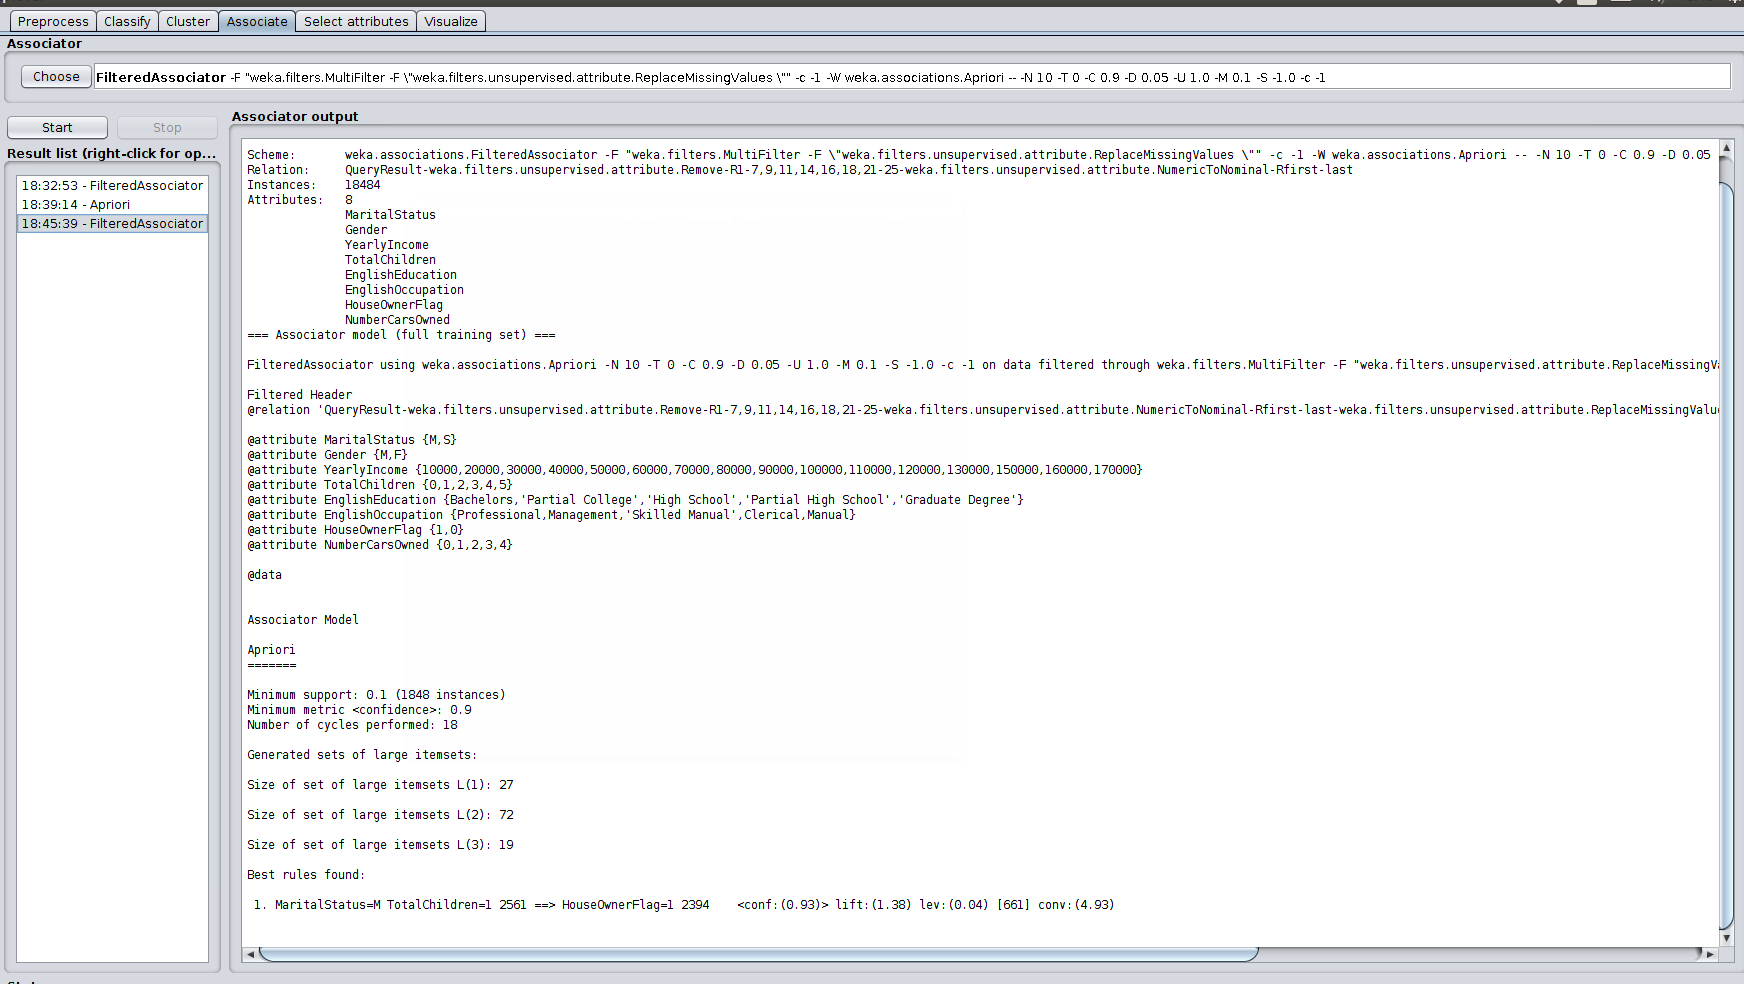
\includegraphics[width=1.3\linewidth, fbox]{img/filtered.png}}%
    \caption{Règles d'associations : FilteredAssociator résultat}
    \label{filtered}
\end{figure}
